\documentclass[runningheads]{llncs}
\usepackage[utf8]{inputenc}

\usepackage{graphicx}
\usepackage{amsmath}
\usepackage{amssymb}
\usepackage{arydshln}
\usepackage{xcolor,ulem}

\usepackage{wrapfig}

% Used for displaying a sample figure. If possible, figure files should
% be included in EPS format.
%
% If you use the hyperref package, please uncomment the following line
% to display URLs in blue roman font according to Springer's eBook style:
% \renewcommand\UrlFont{\color{blue}\rmfamily}

\setlength{\parskip}{0cm}
\setlength{\parindent}{1em}

\newcommand{\reals}{\mathbb{R}}

\newcommand{\comment}[3]{{\color{#1} {\bf #2 :} #3}}
%\newcommand{\comment}[3]{}  % suppress comments
% Use these macros to make comments.
\newcommand{\kui}[1]{\comment{blue}{Kui}{#1}}
\newcommand{\yoav}[1]{\comment{purple}{Yoav}{#1}}
\renewcommand{\beth}[1]{\comment{red}{Beth}{#1}}
\newcommand{\david}[1]{\comment{cyan}{David}{#1}}
\newcommand{\zhongkai}[1]{\comment{brown}{Zhongkai}{#1}}

\renewcommand\floatpagefraction{.99}
\renewcommand\topfraction{.99}
\renewcommand\bottomfraction{.99}
\renewcommand\textfraction{.1}

\setcounter{totalnumber}{50}
\setcounter{topnumber}{50}
\setcounter{bottomnumber}{50}
\setlength{\abovecaptionskip}{0pt}
\setlength{\belowcaptionskip}{0pt}

\title{Towards explainable computer assisted Neuroanatomy}
\author{Kui Qian, Zhongkai Wu, Beth Friedman, David Kleinfeld, Yoav Freund}
\date{May 2022}

\begin{document}

\maketitle

\begin{abstract}
  A fundamental goal of neuroanatomy is the annotation of cells and
  structures.  Manual annotation of structures is based on the spatial
  distribution of cell shape, size, orientation and density.  New
  technology rapid imaging of entire brains at high resolution.
  However, manual identification of structures in these massive
  datasets is prohibitively time consuming.  We present a machine
  learning methodology for developing digital assistants that
  significantly reduce the labor of the anatomist while improving the
  consistency of the annotation.

  Our methodology is based on designing, for each annotation problem,
  a large number of features and using boosting on manually annotated
  images to select the most predictive features.

  We describe two annotation tasks to which we applied this approach.
  The first, more complex task is detecting specific structures in the
  brainstem of the mouse. The second is the detection of individual cells marked
  by a fluorescent dye. We provide the details of both of these
  applications and show that they significantly reduce the anatomist's
  labor in completing these tasks.
  
  %We translate each cell image into a feature vector that
  %includes aspect ratio, orientation and area, as well as additional
  %features derived using a graph Laplacian. The algorithm uses the
  %statistical distribution of these features vectors to identify brain
  %structures.
\end{abstract}

\section{Main}
We propose a system for detecting anatomical structures in the mouse
brain. Our system takes as input high-resolution images of aligned
sections. It produces as output the estimated center of mass (COM) for
each structure. Each detection is assigned a confidence. High
confidence structures are associated with a visual explanation.

\subsubsection {Significance for Neuroscience}
~\\ ~\\
{\bf David and Beth, please expand on the following bullets:}
\begin{itemize}
\item What is Neuroanatomy?
\item Why is Neuroanatomy important (in the context of the great
    advancements in imaging and recording technology)
\item Why is Neuroanatomy hard? (requires a lot of training, the
  number of trained neuroanatomist is small.)
\item An estimate of the amount of manual labor required to achieve
  common tasks.
\item The importance of computer generated confidence and explanations.
\end{itemize}

% Manual neuroanatomical analysis of brain sections is critical for
% creating accurate quantitative results. On the other hand, performing
% neuroanatomical analysis is expensive as it requires many hours of
% work of an expert anatomist.

We consider two labor intensive tasks. Localizing anatomical structure
and counting marked cells. Both tasks involve identifying and marking
locations in images and both require expertise.

A rather obvious but important observation is that while a typical
section will contain hard to identify locations, most of the locations
are easy, in the sense that a person with lesser traing can identify
them reliably.

This observation leads to the following approach to automation. We
use so-called {\em confidence rated detectors}. These detectors
associate with each detection a confidence score. A high confidence
score implies that the example is ``easy''  while the rest are
``hard''. This reduces the workload on the anatomist to the following
tasks:
\begin{itemize}
  \item {\bf Confirming the confident detections} In this step the
    anatomist recieves a small sample of the confident detections and
    verifies that they are correct. The sample size depends on the
    desired accuracy.
    \item {\bf classifiying the unconfident detections} In this step
      the anatomist labels {\em all} of the low confident predictions.
    \item {\bf searching for misses:} In this step the anatomist looks
      for locations that were completely missed by te detector.
  \end{itemize}
  
\subsubsection{Assistive AI} Traditionally, the goal of artificial
  intelligence is to design algorithms which mimic human behavior. AI
  systems are expected to perform as well as humans and, eventually,
  better than humans.

Indeed, in some domains, such as the game of go \cite{silver2017mastering} deep neural
networks (DNN)  have achieved super-human capabilities. In addition,
on highly curated image classification datasets such as ImageNet~\cite{deng2009imagenet} and
CIFAR~\cite{krizhevsky2009learning} DNNs give performance that, some argue, is better than
human. 

However, DNNs have some fundamental drawbacks that limit their
applicability to real-world problems. One problem is that DNNs
require large amounts of training data. In some
setups, such as alpha-go, the labels are generated automatically as
the program plays against itself. When the labels are generated by a
human, as is the case in neuroanatomy, collecting large and reliable
labels is prohibitavely expensive. A second
problem is that the training data and the test data are assumed to
come from the same distribution. However, in most real-world
applications the test data is drawn after the training is complete and
is often generated by a setup that is different from the one used to
collect the training data.
Specifically, in brain imaging, two brain section images from the same
location in different brains are likely to look quite differently.
These images vary for a variety of reasons including: animal to animal variability,
variability in the preparation process, including staining,
sectioning and imaging. In order to create robust classifiers, that do
not need to be retrained on each brain, we need a learning algorithm
that identifies robust patterns that are preserved across brains.
identifies patterns that are consistent across brains.

A third problem arises from variability in human labeling. We use
the term {\em inter rater variation} to refer to the difference in
labels between anatomists. We use the term {\em intra rater
  variation} to refer to the difference in the labels generated by the
same anatomist at different times. Inter and intra rater variations
have been studied in medicine~\cite{gellhorn2013inter}. One
contribution of this paper is an evaluation of rater variation in
neuroanatomy and it's relation to the {\em confident/un-confident}
classifications generated by our methods.

\subsubsection{Boosting and sparse representations}
An important part of the design of any learning algorithm is finding a
representation of input vectors that captures the aspects that are
most relevant for the classification task. Some believe that deep
neural networks can find internal representations autonomously,
without human intervension. However, a close look at the design of
alpha-Go~\cite{silver2017mastering} reveals the high level of human
expertise used to design the features used by the NN.

Boosting~\cite{FreundSc97,schapire2013boosting} is another popular
learning algorithm which combines a large number of so-called ``weak''
rules to construct a single ``strong'' rule. Here we follow an
approach to feature detection for boosting that can be described as
{\em the kitchen sink approach}. This approach starts by constructing
a very large number of potential weak rules. The goal is that a small
subset of the weak rules would provide sufficient information to
perform the classification.

In general, increasing the number of features or rules increases the
danger of over-fitting. However, as has been demonstrated in many
experiments and proven theoretically in~\cite{SchapireFrBaLe98}, the
number of features has only a small influence on overfitting. rather,
it was shown, both theoretically and experimentally, that the {\em
  normalized margin}, which is the difference between the ``+'' votes
and the ``-'' votes for the label of an example, is large.

This justifies the kitchen-sink approach. 


\subsubsection{Boosting and object detection}
The original Adaboost algorithm is designed for the problem of binary
classification. On the other hand, the problems we attack in this
paper are those of {\em object detection} where the object to be
detected is a structure or a marked cell.

In~\cite{violajones01} Viola and Jones demonstrated that boosting
achieves superior speed and accuracy in the task of face detection,
which is now a universal feature in smart phones and cameras.  The
approach used is the pospular {\em sliding-window} approach used in
many other system.  The input to the classifier consists of windows of
different sizes and locations in the image. At the training phase each
window is labeled +1 if it contains the object and 0 if is does
not. At test time the sliding window is used to generate inputs for
the detector and windows that that recieve a high score are defined to
be the predictions.

Viola and jones used so-called {\em Haar features} to represent the
features. The set of features is large ($\sim 10^5$) and was designed
specifically for objects where horizontal and vertical contrasts are
dominant, based on the assumption that faces in photos are usually
upright. This is an example of the {\em kitchen sink} approach where
many features are proposed, but only few are used in the final detector.

We use a very similar design to that of Viola and Jones. We use a 2D
detector to identify marked cells and a 3D detector to identify the 3D
location of a structure in a sectioned brain.
\begin{figure}[t]
  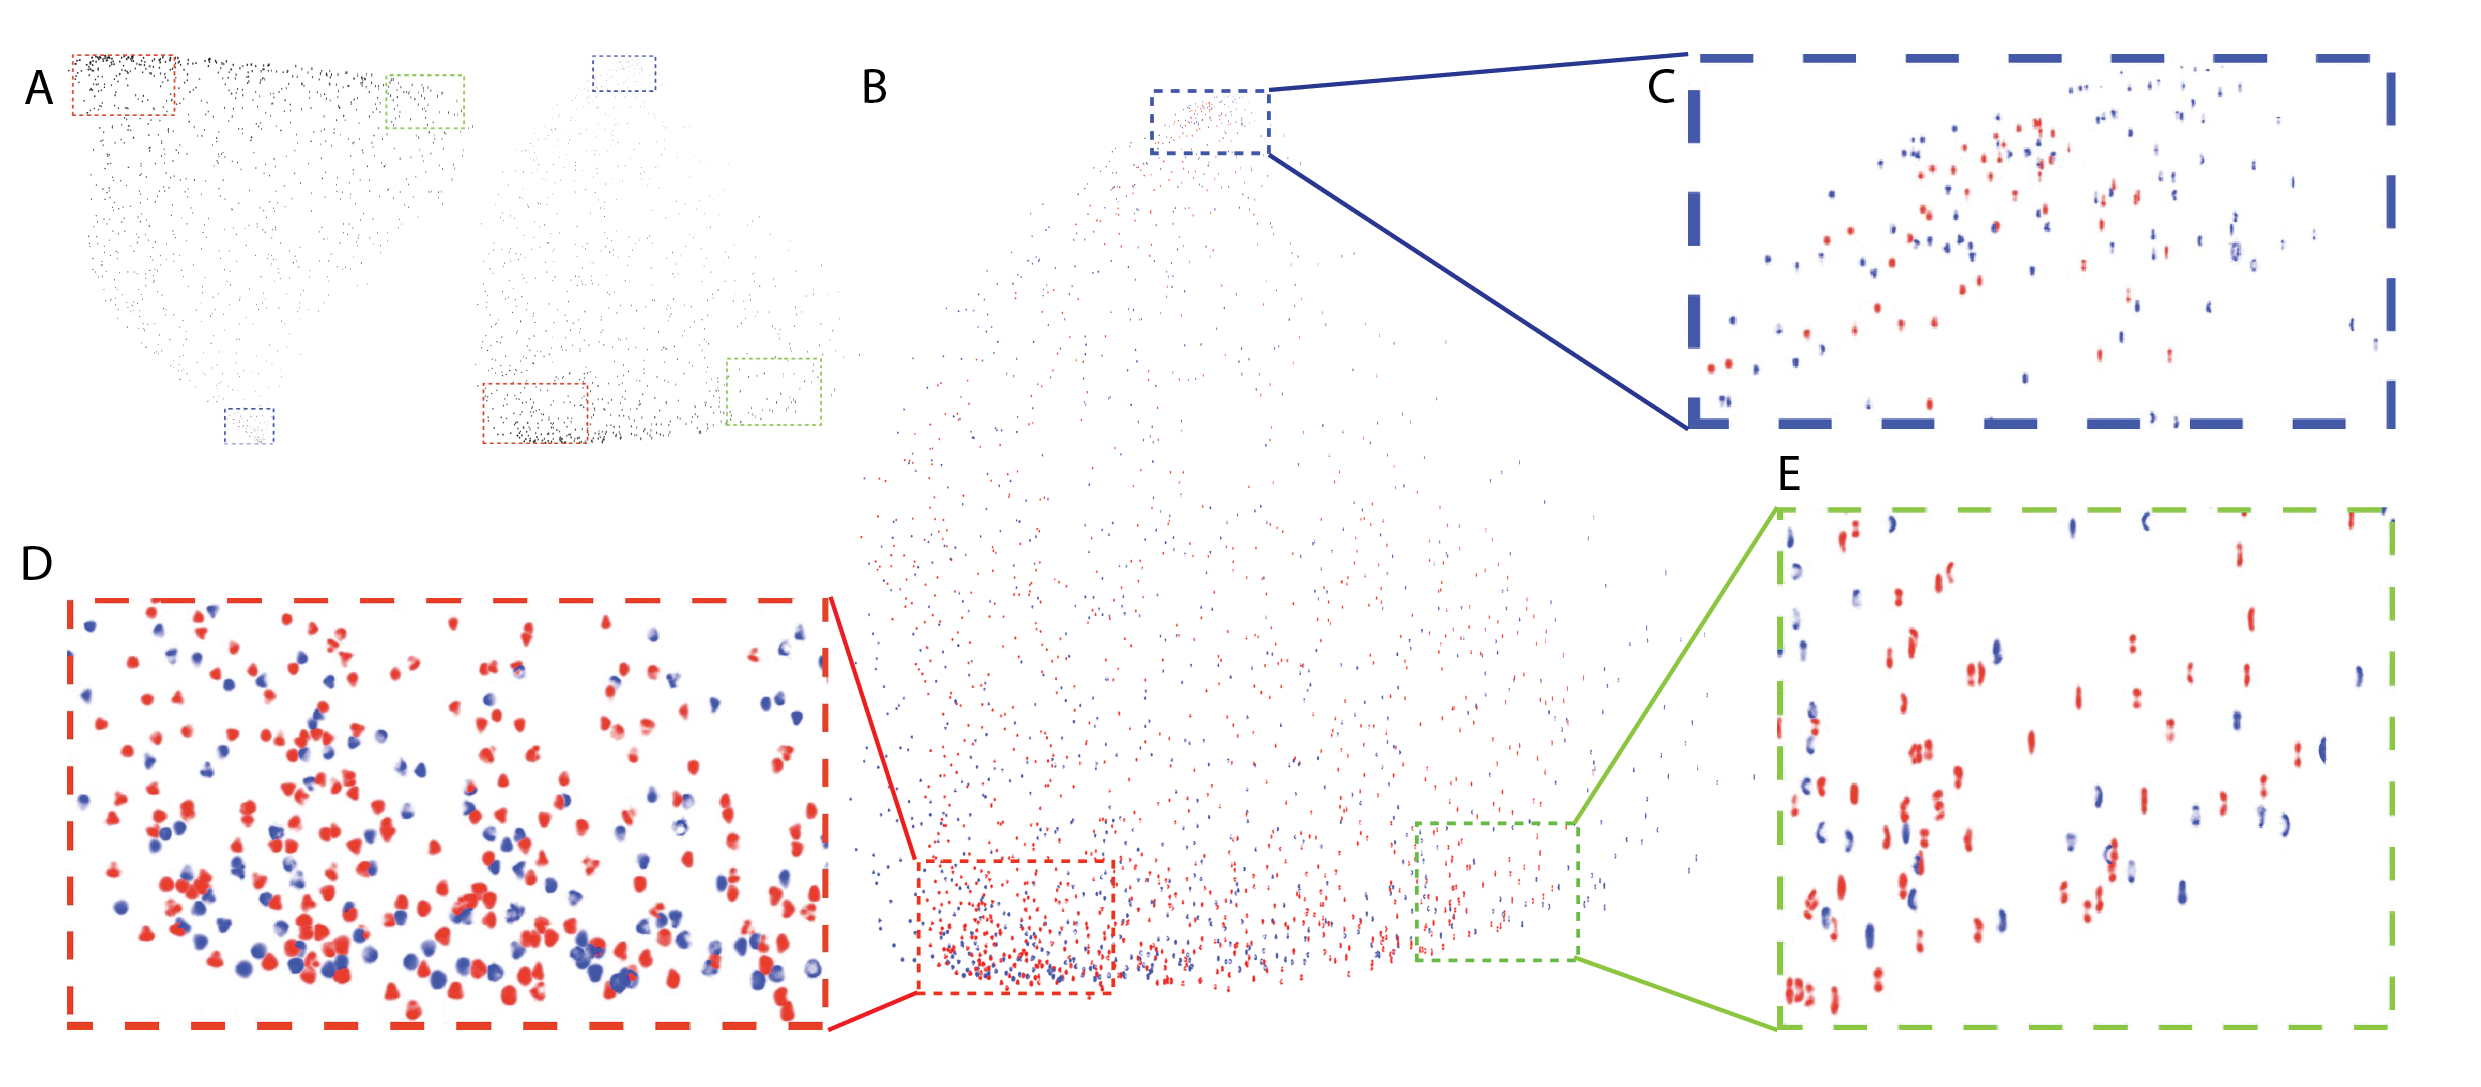
\includegraphics[width=\textwidth]{figures/Diffusionmap.png}
  \caption{{\bf Alignment of diffusion mappings:}  A  presents the similar original cell clouds in diffusion mappings of two brains using different modalities. After transformation, the two cell clouds matched well as shown in B. We marked the three corners of aligned mappings and gave details of these three regions in C, D and E.
}
\end{figure}

\subsubsection{Cell based analysis}

In~\cite{chen2019active} Chen et al used a sliding window and a
Neural network to detect brain structures. The window size is fixed at
$100 \mu m \times 100 \mu m$ which means that a typical window contains 10-100 cells.
The window is used as input to a pre-trained neural network which maps
each window to a vector of 1,000 features. The output layer of
this network is trained using logistic regression. The earlier layers
are fixed. Chen et al used this system to demonstrate the first
structure detection that operates at the resolution of single cells.
However, the concept of a cell is not directly used by this as the
input to the neural network consists of raw pixel values, and not any
higher-order features.

On the other hand, anatomist base their analysis on cytoarchitecture,
which, in turn, is based on the shapes of individual cells and the
relationshp between them. This makes it harder for the anatomist to
understand the decisions of the detector.

To remedy this problem and make the detections explainable, we use
features that are based on the shapes of individual cells.

\section{Results}

\subsection{Detecting Structures}

\subsubsection{Adaptive Cell shape parametrization} Uses a combination of Hu moments and dimensionality reduction using eigen-maps.
Eigen-maps learn a dimensionality reducing mapping cell shape to a ten dimensional representation.
As it is an unsupervised method it requires no human labeling. We take advantage of the very large number of cells in single brain. 

\subsubsection{Structure detection accuracy}
In figure~(\ref{fig:structureAccuracy}) we show the error of our
detector as a function of the detection confidence. 
\begin{figure}[t]
  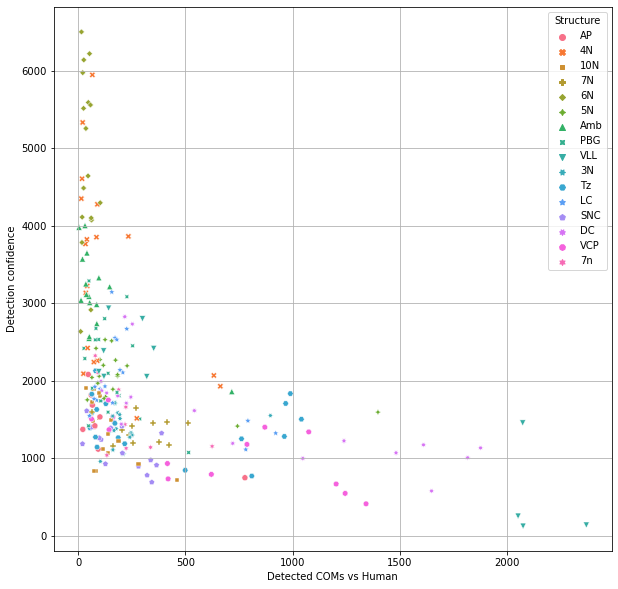
\includegraphics[width=0.65
  \textwidth]{figures/ErrorVsConfidence.png}
  \hspace{1cm}
  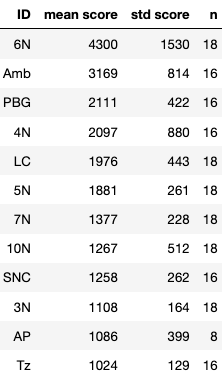
\includegraphics[width=0.25\textwidth]{figures/ScoresOfStructures.png}
  \caption{\label{fig:structureAccuracy} {\bf Evaluation of detection
      accuracy:} A shows the relationship between detection confidence
    and the detection error relative to human annotation.}
\end{figure}

\begin{figure}[b]
  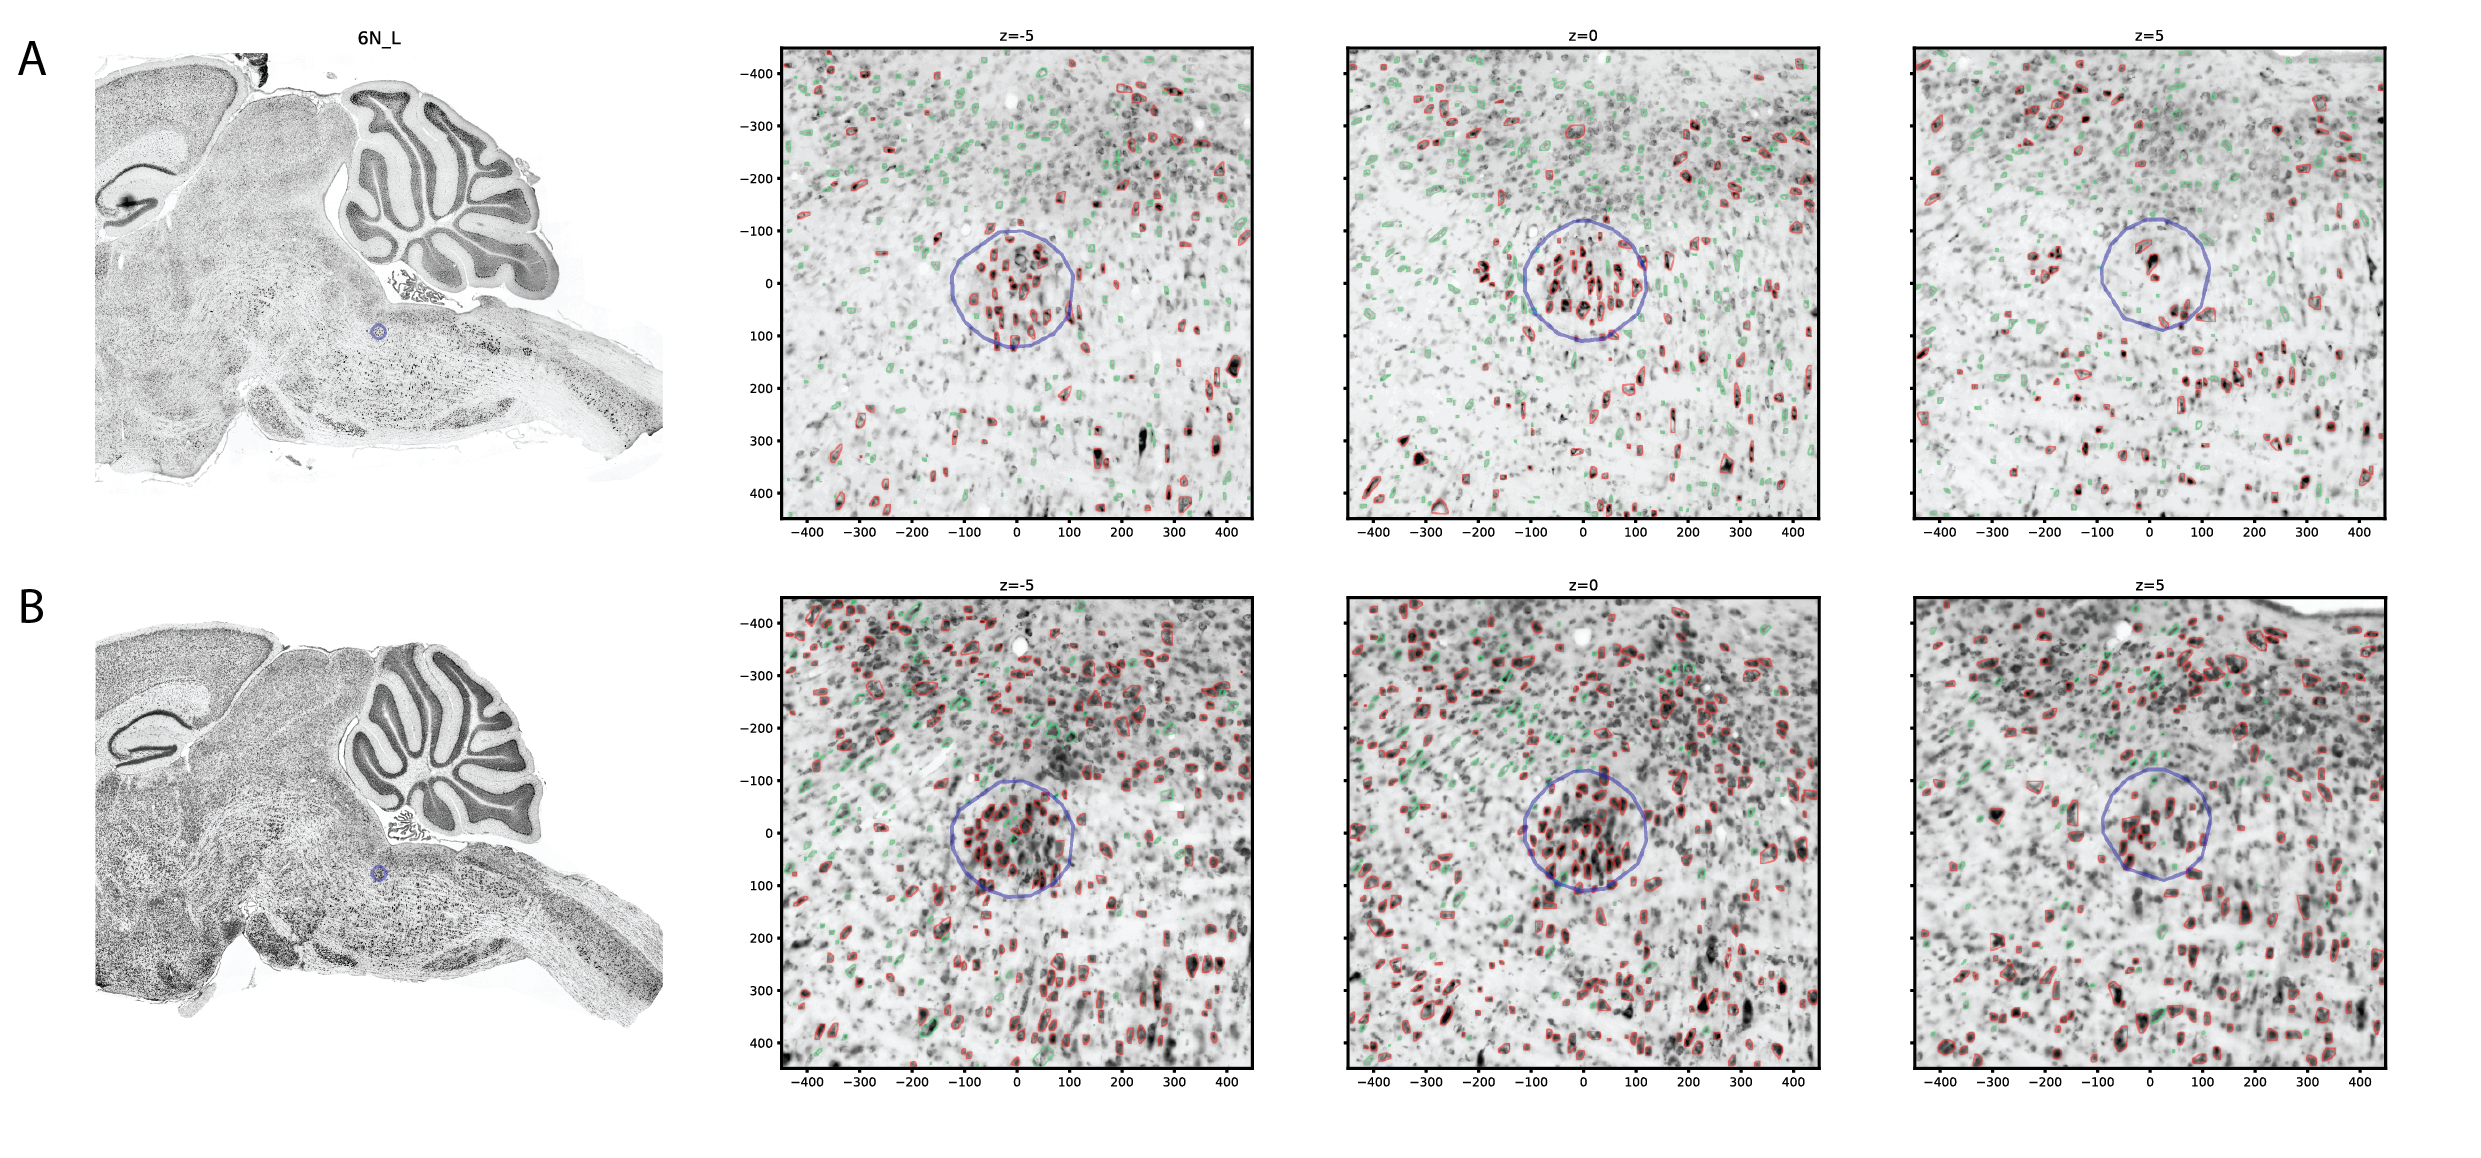
\includegraphics[width=\textwidth]{figures/DetectionExplanation.png}
  \caption{\label{fig:explaining} {\bf explaining detections:} visual explanations for the
    detection of 6N\_L in two brains. A and B are brain images of two
    brains at section z=0, marking the locations of 6N\_L with blue
    contours and showing cell distributions of the top 3 important
    features for regions inside and outside the contours.  The cells
    come from three sections, 100 microns apart. The red marked cells
    are evidence of the inside of the structure, the green cells,
    which are much smaller, are evidence of the outside. Note that
    section z=5 has very few cells. The detector overcomes this by
    combining information from all sections.  The bottom brain is
    stained darker than the top one, which is likely to confuse a
    method that is not cell based.}
  \end{figure}

\subsubsection{Explaining detections}
For each detection we generate an explanation. The explanation
consists of an annotated image in which cells that are typical of the
structure and cells that are typical of the region outside the
structure are highlighted. Figure~(\ref{fig:explaining}.)


\subsection{Detecting marked cells}

\begin{figure}[t]
  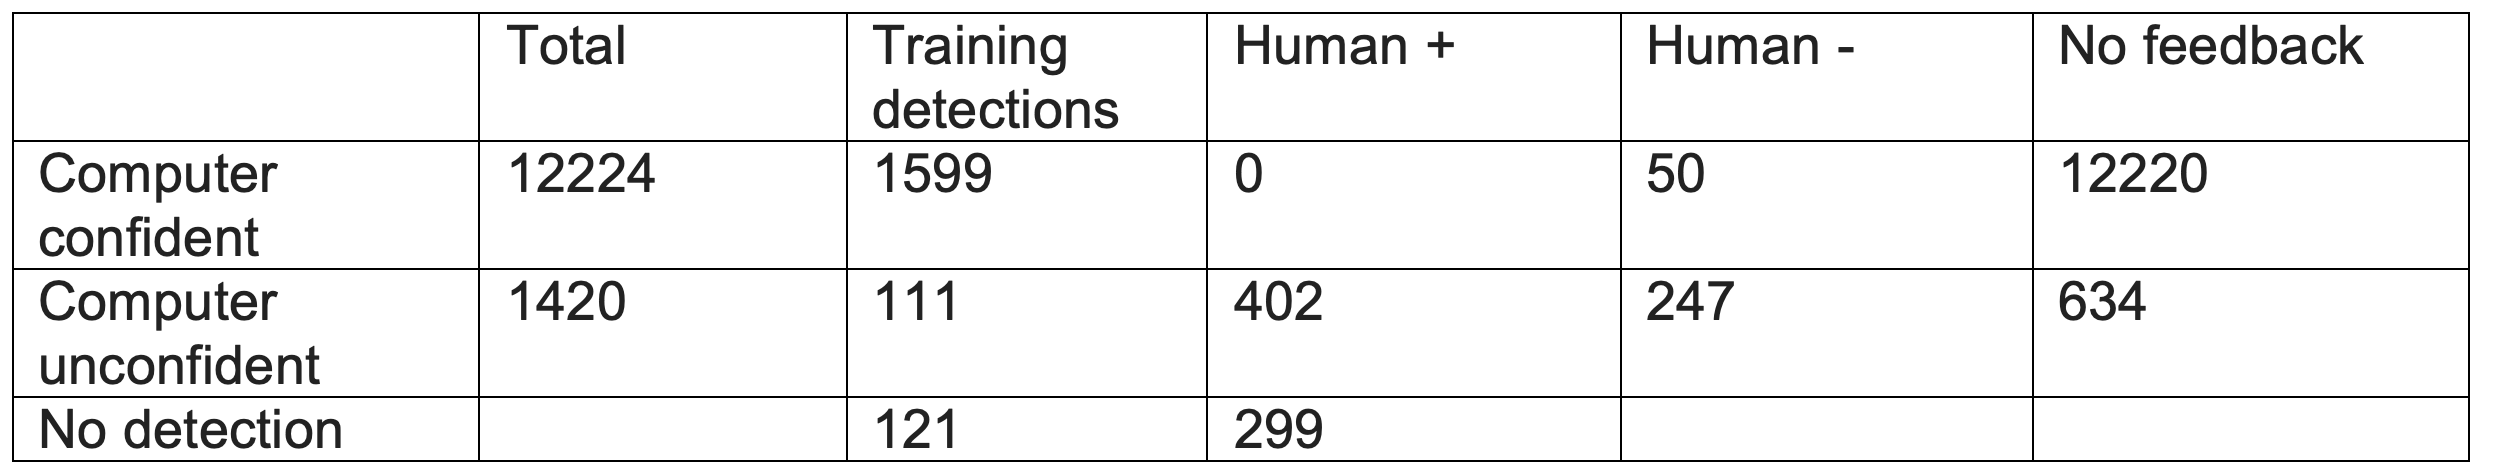
\includegraphics[width=\textwidth]{figures/MarkedCellsDetectionNumbers.png}
\end{figure}

\begin{figure}[b]
  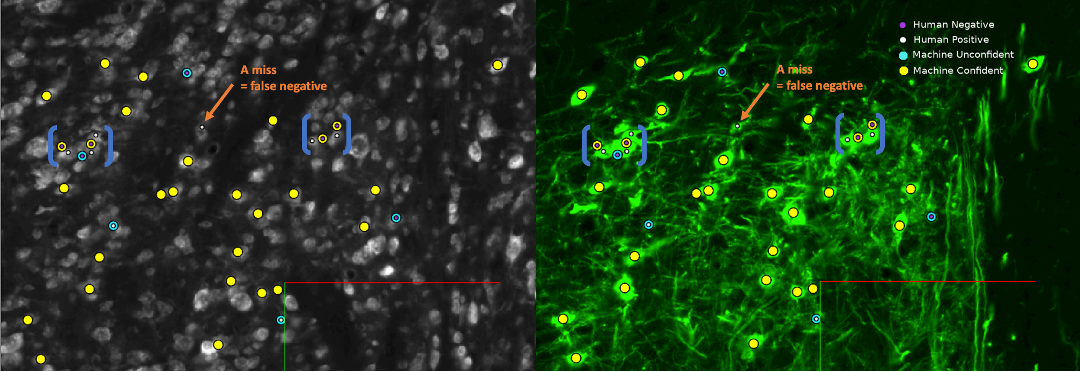
\includegraphics[width=\textwidth]{figures/Marked_cell_detections.png}
  \caption{}
\end{figure}

\iffalse
\begin{itemize}
\item The amount of manual work that it takes to manually mark cells.
\item inter-rater and intra-rater disagreement rate.
\item How to count false detections "with approximately correct
  detections detection".
\item How to quantify reduced mental load of QA vs detection.
\end{itemize}
\fi
\newpage

\section{Methods}

\subsection{Structure Detection}

\iffalse
\begin{figure}[t]
  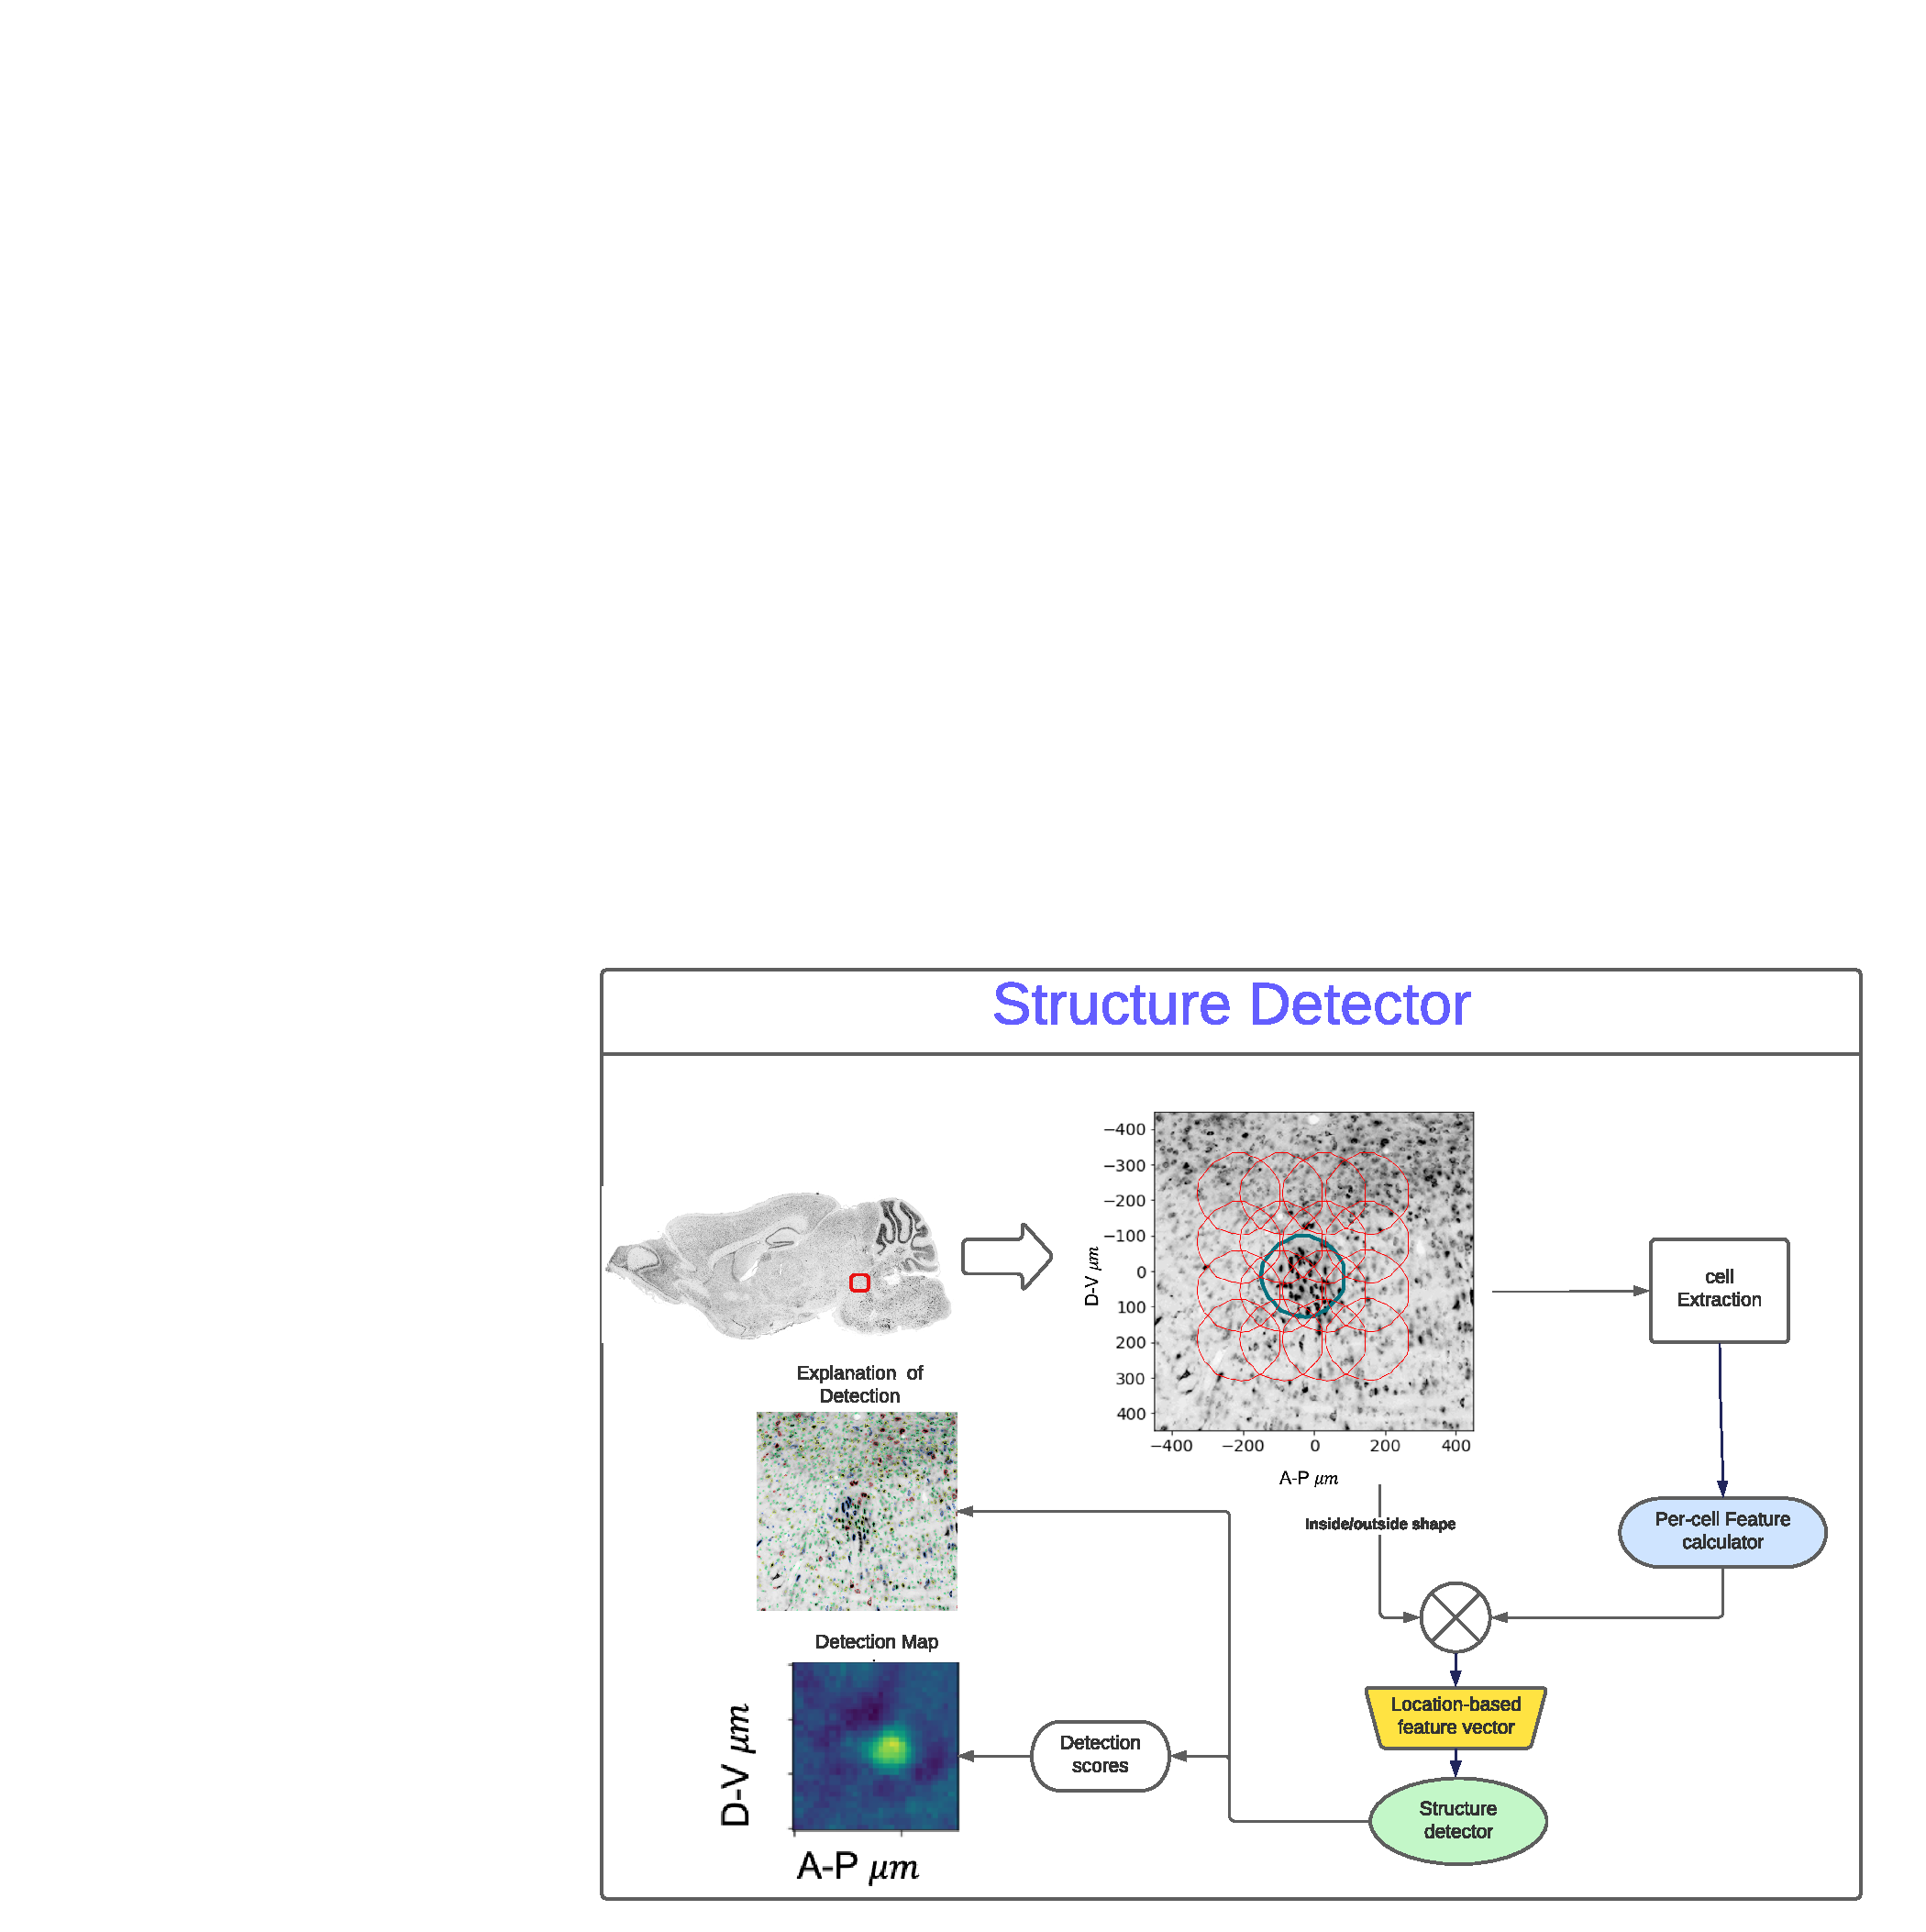
\includegraphics[width=\textwidth]{figures/detection.pdf}
  \caption{Detecton \label{fig:detection}}
\end{figure}

\begin{figure}[t]
  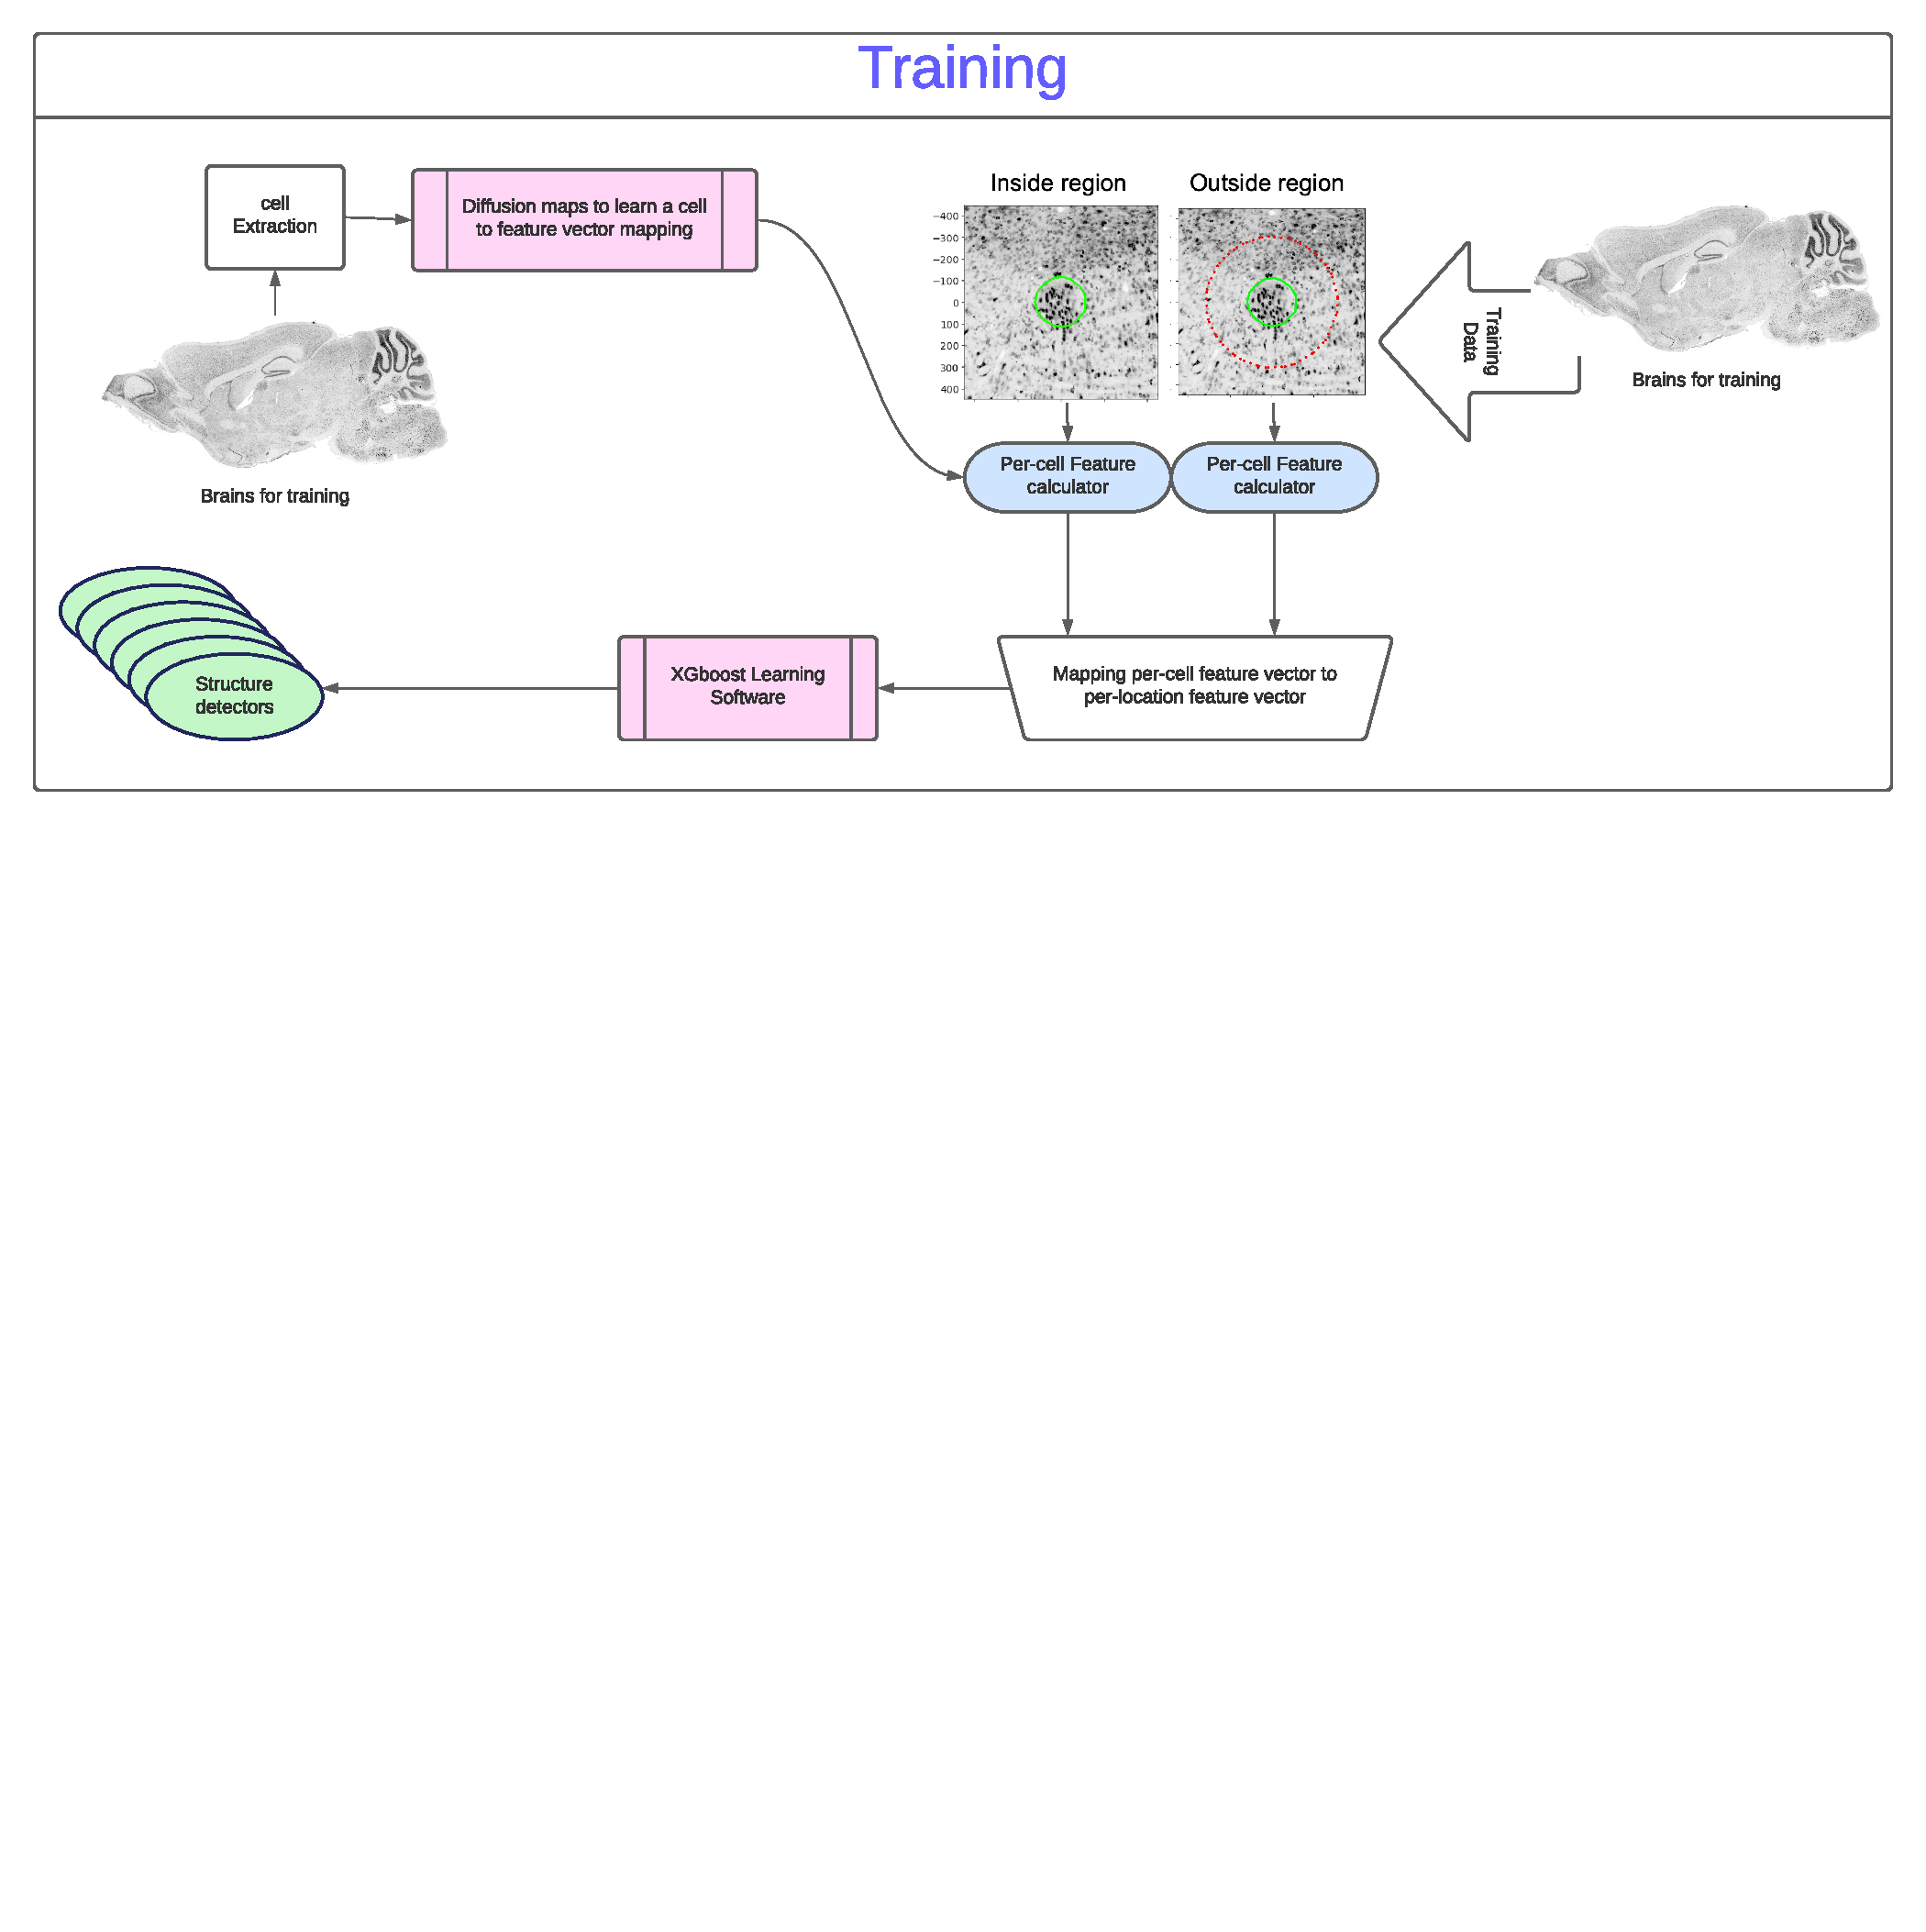
\includegraphics[width=\textwidth]{figures/Training.pdf}
  \caption{Training \label{fig:training}}
\end{figure}
\fi

\begin{figure}[t]
  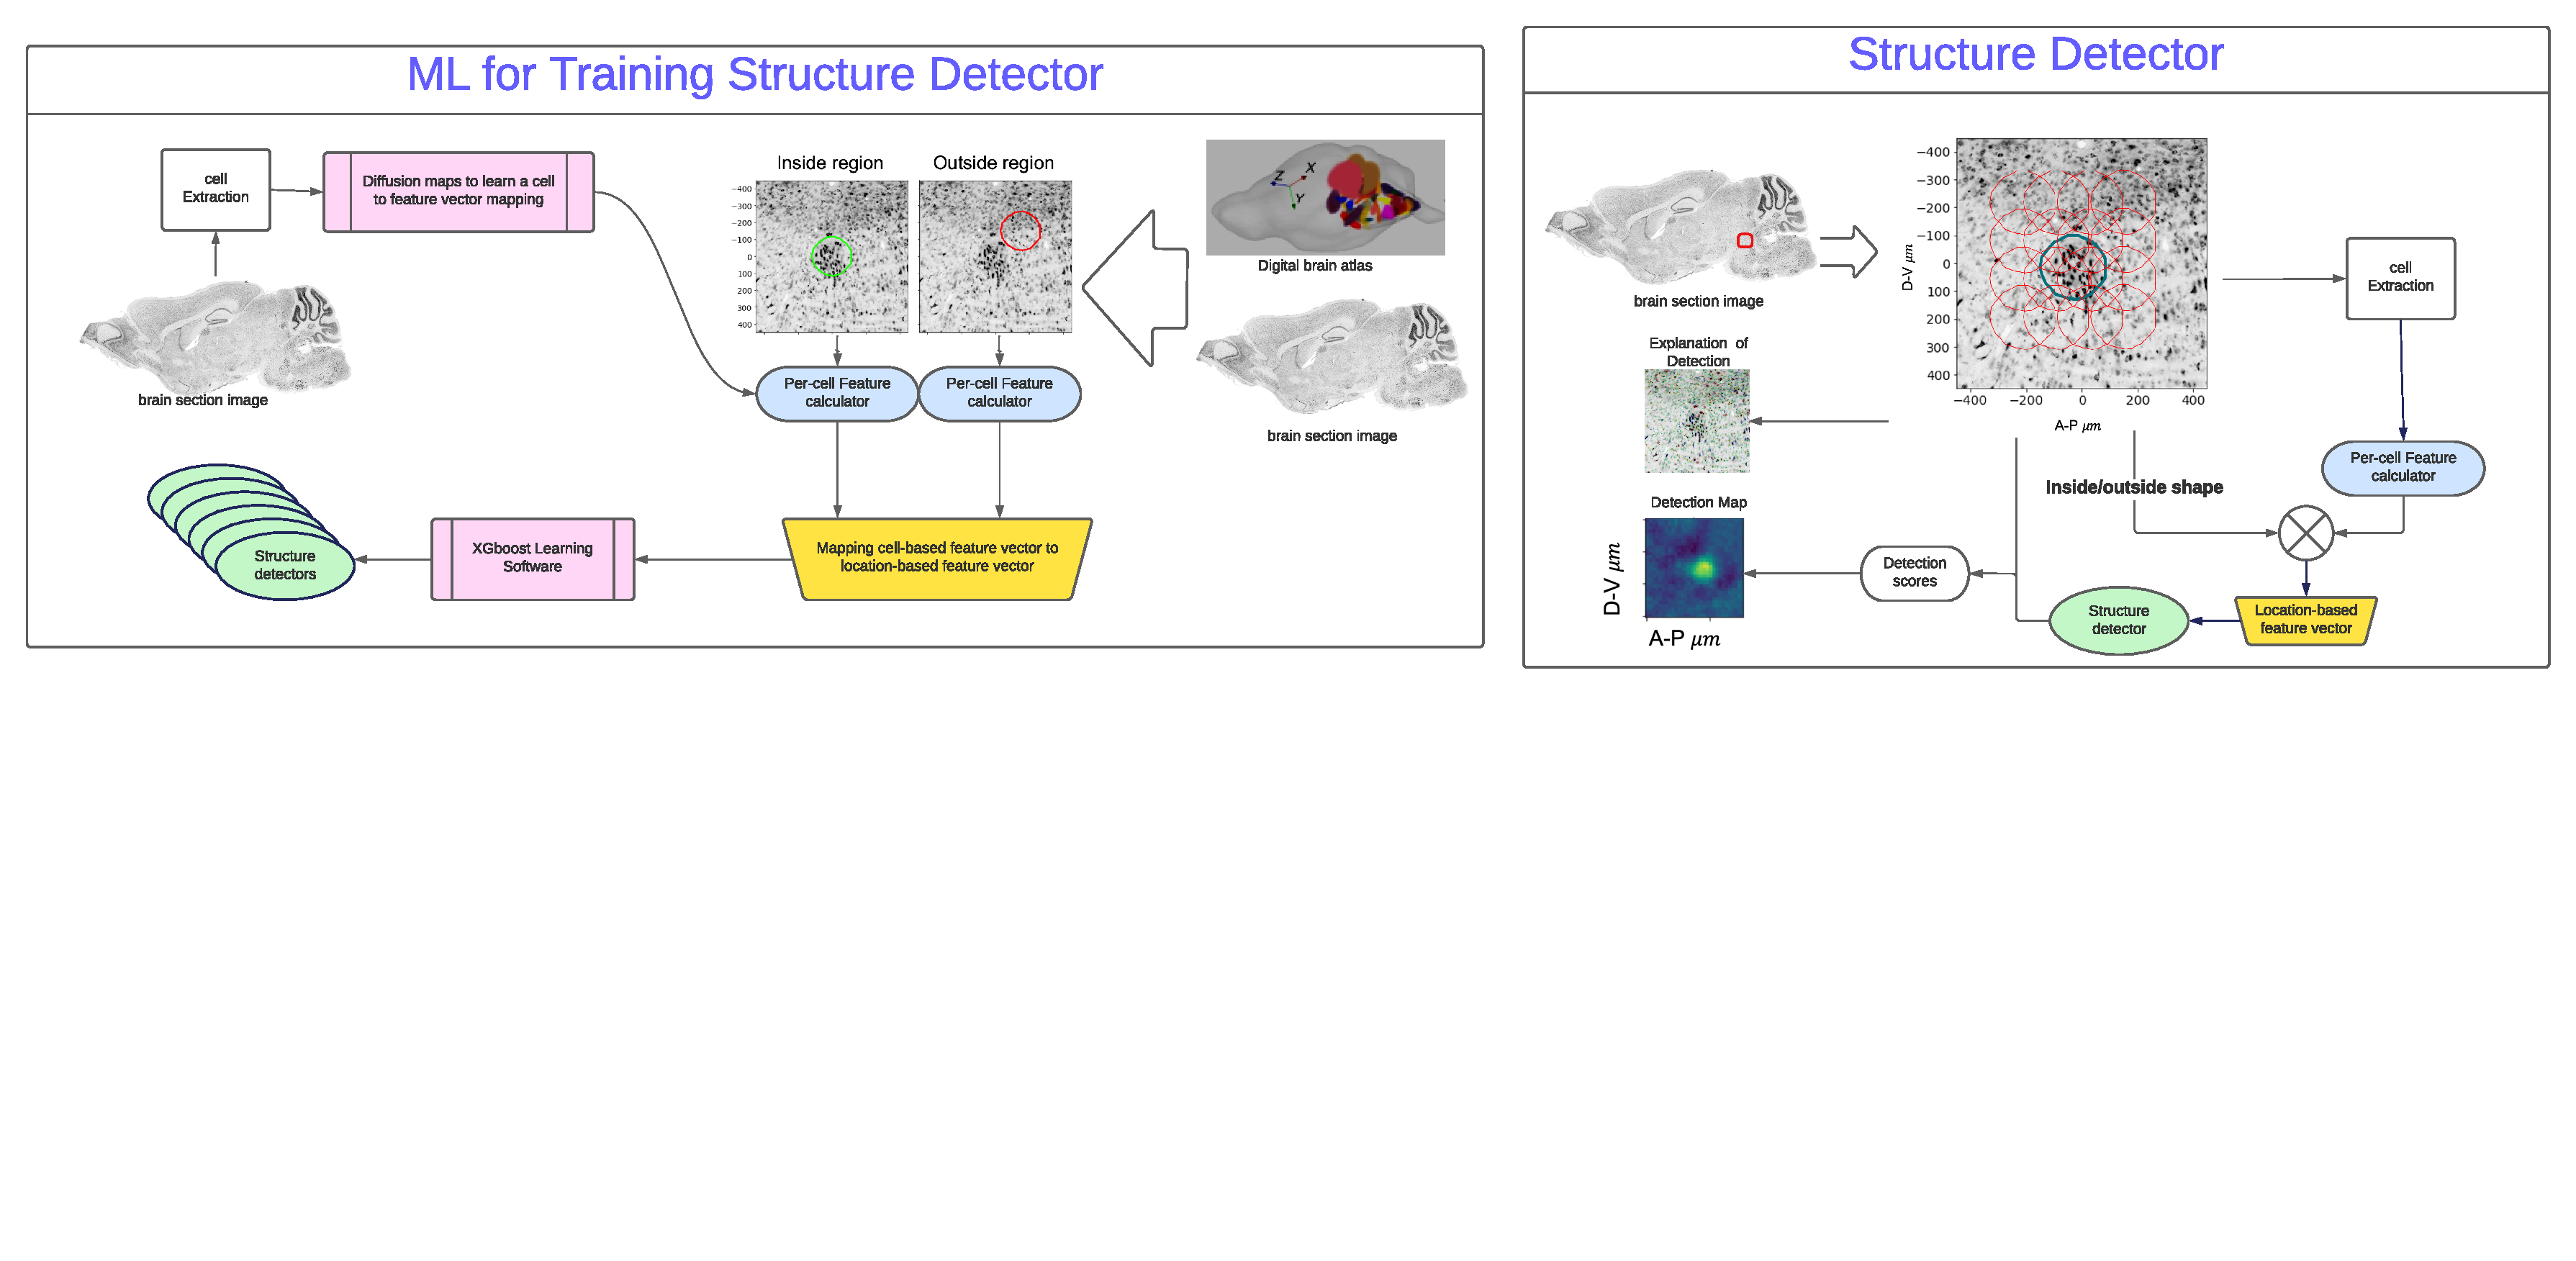
\includegraphics[width=\textwidth]{figures/architecture.pdf}
  \caption{System architecture \label{fig:architecture}}
\end{figure}

The design of the structure detector system is described in Figure~\ref{fig:architecture}.
The system consists of two subsystems: the structure detector whose
function is to determine the location os brain structure, and the ML
subsystem which uses machine learning to create the structure detector.

The subsystems are further devided into components, so of which
are common to the two subsystems. We describe each of those components
in turn.

%\subsection{System Inputs}
To train the detectors we combine three sources of information:
\begin{itemize}
    \item {\bf Images of aligned sections:} The Nissl images of XX brains are the primary information source. They are also by far the largest at XXX GB per brain.
    \item {\bf The Atlas} is a representation of the shape of each structure and the relative locations of the structures. The atlas was constructed through a concensus ....
    \item {\bf COMs for individual brains:} For XX brains we had an anatomist locate the COM ....
\end{itemize}

\begin{enumerate}
\item{\bf Cell extraction and shape parametrization}
An image of a single cell is typically around 50$\times$50 pixels, or a 2500 dimensional vector. The dimension of this representation is too high for effective machine learning. We therefor seek a dimensionality reduction mapping. This mapping consists of three parts:
\begin{enumerate}
    \item {\bf Normalization:} We normalize the image of the cell in three ways. We 
    shift the grey-levels so that the mean is XXX, scale the grey levels so that the standard deviation is YYY, and rotate the image so that the long axis of the cell is in angle zero. The three parameters associated with the normalizations define three features.
    \item {\bf Standard shape features}: we use the Hu features: x,y,z...
    \item{ \bf Diffusion maps}: Diffusion
      Mapping~\cite{belkin2003,coifman2005geometric} is a non-linear
      dimensionality reduction method that is based on a graphical
      representation of the data and on the Laplace operator on
      graphs.
      \end{enumerate}
\end{enumerate}
\subsubsection{ Characterizing Cytoarchitecture} uses Difference between the CDFs for inside and outside of each structure (based on manually annotated structure boundaries). 
\subsubsection { Structure detectors} Combine the difference-of-CDF
features using boosted trees (XGBoost). Each structure has a
corresponding detector.

\subsubsection { Structure detection confidence} The confidence of structure
  detections is measured by the prediction margin and by the sharpness
  of the detection peak.

\subsubsection { Structure detection explanation}

\iffalse
which is based on cells as the basic unit. Doing so provides an explanation for the detector's decision. We use unsupervised learning to find a dimensionality reducing mapping for cell shapes. We make efficient use of manual annotations by estimating the shape of each structure from a few brains and anatomists. We leverage this information in the detector training by having the anatomist identify the location of the center of mass for each structure.
\fi


\begin{itemize}
\item Cell based features.
\item Diffusion mapping.
\item Calibration of the diffusion features.
\item Region features and CDFs.
\item Boosting and XGBoost.
\item Localizing structures. Rough alignment, computing detections
  scores, computing autocorrelation and asigning confidence.
\item Using the system for brain-to-atlas alignment.
\item Generating explanations.
\end{itemize}

 \bibliographystyle{splncs04}
 \bibliography{Reference,bib}



\end{document}


